% Este trabalho está licenciado sob a Licença Atribuição-CompartilhaIgual 4.0 Internacional Creative Commons. Para visualizar uma cópia desta licença, visite http://creativecommons.org/licenses/by-sa/4.0/deed.pt_BR ou mande uma carta para Creative Commons, PO Box 1866, Mountain View, CA 94042, USA.

\chapter{Linguagem de Programação}\label{cap_lingua}
\thispagestyle{fancy}

\section{Computador}\label{cap_lim_sec_computador}

\begin{flushright}
  [YouTube] | [Vídeo] | [Áudio] | [Contatar]
\end{flushright}

Um computador\footnote{Consulte \href{https://pt.wikipedia.org/wiki/Computador}{Wikipédia: Computador} para uma introdução sobre a história e outras questões sobre computadores.} é um \emph{sistema computacional} de elementos físicos (\emph{hardware}) e elementos lógicos (\emph{software}).

O \emph{hardware} são suas partes mecânicas, elétricas e eletrônicas como: fonte de energia, teclado, mouse/painel tátil, monitor/tela, dispositivos de armazenagem de dados (HDD, {\it hard disk drive}; SSD, {\it solid-state drive}; RAM, {\it random-access memory}; etc.), dispositivos de processamento (CPU, {\it central processing unit}, GPU, {\it graphics processing unit}), conectores de dispositivos externos (microfone, caixa de som, fone de ouvido, USB, etc.), placa mãe, etc..

O \emph{software} é toda a informação processada pelo computador, qualquer código executado e qualquer dado usado nas computações.

\begin{figure}[H]
  \centering
  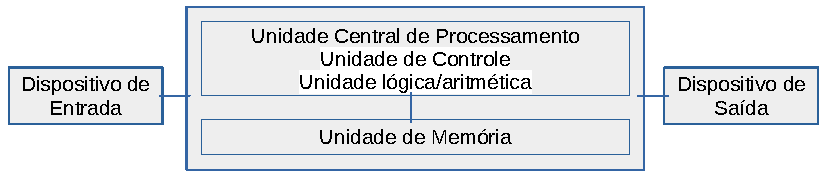
\includegraphics[width=\textwidth]{./cap_lingua/dados/fig_arqVonNeumann/main}
  \caption[Arquitetura de von Neumann]{Arquitetura de computador de von Neumann.}
  \label{cap_lim_sec_computador:fig:arqVonNeumann}
\end{figure}

Os computadores que comumente utilizamos seguem a arquitetura de John von Neumann\footnote{John von Neumann, 1903 - 1957, matemático húngaro, naturalizado estadunidense. Fonte: \href{https://pt.wikipedia.org/wiki/John_von_Neumann}{Wikipédia}.}, que consiste em dispositivo(s) de entrada de dados, unidade(s) de processamento, unidade(s) de memória e dispositivo(s) de saída de dados (Figura~\ref{cap_lim_sec_computador:fig:arqVonNeumann}).

\begin{itemize}
\item \emph{Dispositivos de entrada e saída}

  São elementos do computador que permitem a comunicação humana (usuária(o)) com a máquina.

  \begin{itemize}
  \item \emph{Dispositivos de entrada}

    São elementos que permitem o fluxo de informação da(o) usuária(o) para a máquina. Exemplos são: teclado, mouse/painel tátil, microfone, etc.

  \item \emph{Dispositivos de saída}

    São elementos que permitem o fluxo de informação da máquina para a(o) usuária(o). Exemplos são: monitor/tela, alto-falantes, luzes espia, etc.
  \end{itemize}

\item \emph{Unidade central de processamento}

  A \emph{CPU} (do inglês, {\it Central Processing Unit}) é o elemento de processa as informações e é composta de \emph{unidade de controle}, \emph{unidade lógica e aritmética} e de \emph{memória cache}.

  \begin{itemize}
  \item \emph{Unidade de controle}

    Coordena as execuções do processador: busca e decodifica instruções, lê e escreve no {\it cache} e controla o fluxo de dados.

  \item \emph{Unidade lógica/aritmética}

    Executa as instruções operações lógicas e aritméticas, por exemplo: executar a adição, multiplicação, testar se dois objetos são iguais, etc.

  \item \emph{Memória cache}

    Memória interna da CPU muito mais rápida que as memórias RAM e dispositivos e armazenamento HDD/SDD. É um dispositivo de memória de pequena capacidade e é utilizada como memória de curto prazo e diretamente acessada.
  \end{itemize}

\item \emph{Unidades de memória}

  As unidades de memória são elementos que permitem o armazenamento de dados/objetos. Como memória principal tem-se a \emph{ROM} (do inglês, {\it Read Only Memory}) e a \emph{RAM} (do inglês, {\it Random Access Memory}) e como memória de massa/secundária tem-se HDD, SSD, entre outras.

\item \emph{Memória ROM}

  A memória ROM é utilizada para armazenamento de dados/objetos necessários para dar início ao funcionamento do computador. Por exemplo, é onde a BIOS (dos inglês, {\it Basic Input/Output System}, Sistema Básico de Entrada e Saída) é armazenada. Ao ligarmos o computador este programa é iniciado e é responsável por fazer o gerenciamento inicial dos diversos dispositivos do computador e carregar o \emph{sistema operacional} (conjunto de programas cuja função é de gerenciar os recursos do computador).

\item \emph{Memória RAM}

  Memória de acesso rápido utilizada para dados/objetos de uso frequente durante a execução de programas. É uma memória volátil, i.e. toda a informação guardada nela é perdida quando o computador é desligado.

\item \emph{Memória de massa/secundária}

  Memória de massa ou secundária são usadas para armazenar dados/objetos por período longo. Normalmente, são dispositivos HDD ou SDD, os dados/objetos são guardados mesmo que o computador seja desligado e contém grande capacidade de armazenagem.   
\end{itemize}

Os \emph{software} são os elementos lógicos de um sistema computacional, são programas de computadores que contém as instruções que gerenciam o \emph{hardware} para a execução de tarefas específicas, por exemplo, imprimir um texto, gravar áudio/vídeo, resolver um problema matemático, etc. Programar é o ato de criar programas de computadores.

As informações fluem no computador codificadas como registros de {\it bits}\footnote{Usualmente de tamanho $64$-{\it bits}.} (sequência de zeros ou uns). Há registros de instrução e de dados. Programar diretamente por registros é uma tarefa muito difícil, o que levou ao surgimento de linguagens de programação. Uma \emph{linguagem de programação}\footnote{Código de programação, código de máquina ou linguagem de máquina.} é um método padronizado para escrever instruções para execução de tarefas no computador. As instruções escritas em uma linguagem são interpretadas e/ou compiladas por um software (interpretador ou compilador) da linguagem que decodifica as instruções em registros de instruções e dados, os quais são efetivamente executados na máquina.

\subsection{Exercícios Resolvidos}

\emconstrucao

\subsection{Exercícios}

\emconstrucao

\section{Linguagem de Programação}\label{cap_lingua_sec_lingua}

\emconstrucao

\subsection{Exercícios Resolvidos}

\emconstrucao

\subsection{Exercícios}

\emconstrucao
